\IfFileExists{optica-article.cls}{%
  \documentclass{optica-article}%
}{%
  \documentclass{../optica-article}%
}
\journal{opticajournal}
\usepackage{graphicx}
\graphicspath{{./}{../}}

\begin{document}

\title{Supplement 1: Supporting content}

\renewcommand{\thefigure}{S\arabic{figure}}
\renewcommand{\thetable}{S\arabic{table}}
\renewcommand{\theequation}{S\arabic{equation}}

%% ============================================================
\section*{Appendix A. Theoretical derivations}

\subsection*{A.1 Finite-$M$ Airy crosstalk: closed form and large-$M$ limit}

For $M$ uniformly spaced target modes in a cavity of finesse $\mathcal{F}$, the general-finesse form of the Airy circular sum used in the main text is
\begin{equation}
P_{\mathrm{noise}}^{(M)}(\mathcal{F})
=\sum_{n=1}^{M-1}
\frac{1}{1+\left(\dfrac{2\mathcal{F}}{\pi}\right)^{\!2}\sin^2\!\!\left(\dfrac{\pi n}{M}\right)}.
\label{eq:supp_pnoise_airy}
\end{equation}
With $a=(2\mathcal{F}/\pi)^2$, this sum can be evaluated in closed form using the standard trigonometric-sum identity
\begin{equation}
\sum_{n=0}^{M-1}\frac{1}{1+a\sin^2(\pi n/M)}
=\frac{M}{\sqrt{1+a}}\,\frac{1+q^M}{1-q^M},
\label{eq:supp_trig_identity}
\end{equation}
This identity is valid for $a>0$, with $q=(\sqrt{1+a}-1)/(\sqrt{1+a}+1)$ and $0<q<1$. The crosstalk sum in Eq.~(\ref{eq:supp_pnoise_airy}) excludes the $n=0$ contribution, which is unity. Subtracting this contribution yields the closed-form expression
\begin{equation}
P_{\mathrm{noise}}^{(M)}(\mathcal{F})
=\frac{M}{\sqrt{1+a}}\,\frac{1+q^M}{1-q^M}-1.
\label{eq:supp_pnoise_closed}
\end{equation}
The corresponding extinction ratio and sorting efficiency are
\begin{equation}
\mathrm{ER}_{\mathrm{sum}}^{(M)}=10\lg\frac{1}{P_{\mathrm{noise}}^{(M)}},
\qquad
\eta_{\mathrm{sort}}^{(M)}=\frac{1}{1+P_{\mathrm{noise}}^{(M)}}.
\label{eq:supp_er_eta}
\end{equation}

\medskip\noindent\textbf{Capacity-boundary specialization and large-$M$ limit.}\quad
At the capacity-boundary finesse $\mathcal{F}=M\tau_0$, the sharpness parameter becomes $a_M=(2M\tau_0/\pi)^2$. As $M\to\infty$ at fixed $\tau_0$, $a_M\to\infty$ and $\sqrt{1+a_M}\sim 2M\tau_0/\pi$. Thus, the prefactor satisfies $M/\sqrt{1+a_M}\to\pi/(2\tau_0)$. For $q_M=q|_{a=a_M}$, the large-$M$ expansion gives $q_M\approx 1-2/\sqrt{a_M}=1-\pi/(M\tau_0)$, and therefore $(q_M)^M\to e^{-\pi/\tau_0}$. Substitution into Eq.~(\ref{eq:supp_pnoise_closed}) yields
\begin{equation}
P_{\mathrm{noise}}^{(\infty)}(\tau_0)
=\frac{\pi}{2\tau_0}\,\frac{1+e^{-\pi/\tau_0}}{1-e^{-\pi/\tau_0}}-1
=\frac{\pi}{2\tau_0}\coth\frac{\pi}{2\tau_0}-1.
\label{eq:supp_pnoise_limit}
\end{equation}
At $\tau_0=3$, Eq.~(\ref{eq:supp_pnoise_limit}) gives $P_{\mathrm{noise}}^{(\infty)}\approx 0.0898$. The corresponding system extinction ratio and sorting efficiency are $\mathrm{ER}_{\mathrm{sum}}^{(\infty)}\approx 10.47\,\mathrm{dB}$ and $\eta_{\mathrm{sort}}^{(\infty)}\approx 91.76\%$, respectively, consistent with Table~1 in the main text. The finite-$M$ Airy sum approaches this limit from below, so the large-$M$ expression provides a conservative upper bound on the crosstalk: $P_{\mathrm{noise}}^{(M)}<P_{\mathrm{noise}}^{(\infty)}$ for all finite $M$.

\medskip\noindent\textbf{Numerical evaluation at $M=9$.}\quad
Evaluating Eq.~(\ref{eq:supp_pnoise_closed}) at the threshold finesse $\mathcal{F}_{\min}=27$ gives $\mathrm{ER}_{\mathrm{sum}}^{(9)}=10.53\,\mathrm{dB}$ and $\eta_{\mathrm{sort}}^{(9)}=91.9\%$. This value lies within $0.06\,\mathrm{dB}$ of the conservative large-$M$ limit and corresponds to the $M=9$ row in Table~2 of the main text. At the measured finesse $\mathcal{F}=32.21$, the same expression gives $\mathrm{ER}_{\mathrm{sum}}^{(9)}=12.04\,\mathrm{dB}$, matching the finite-$M$ Airy reference used in the main text.

%% ============================================================
\subsection*{A.2 Optimal geometry for general target sets: rationality proof}

For a general target set $S=\{N_1,\dots,N_M\}$, define the pairwise order-difference set as $D(S)=\{N_j-N_i:i<j\}$. The minimum folded spacing is
\begin{equation}
s_{\min}(k;S)=\min_{d\in D(S)}\|d\,k\|,
\label{eq:supp_smin_general}
\end{equation}
where $\|x\|=\min_{n\in\mathbb{Z}}|x-n|$ denotes the distance from $x$ to its nearest integer. The design task is to find the value $k^*$ that maximizes $s_{\min}(k;S)$ over a rational search interval $I=[a,b]$.

For each difference $d\in D(S)$ and each integer $n$, the function $|dk-n|$ is a V-shaped piecewise-linear function of $k$ with vertex at $k=n/d$. Over the finite interval $I$, only finitely many integers $n$ are relevant. Therefore, $s_{\min}(k;S)$ is the pointwise minimum of finitely many such V-profiles and hence a piecewise-linear lower envelope.

On any linear segment of the lower envelope, the slope is nonzero. An interior maximum therefore cannot occur within such a segment; the global maximum must occur at a breakpoint or at an endpoint of $I$. The relevant breakpoints are of two types: (i)~V-profile vertices $n/d$, which are rational with denominator at most $D_{\max}=\max D(S)$; and (ii)~intersections of two V-profiles with slopes $+d_1$ and $-d_2$, which give $k=(n_1+n_2)/(d_1+d_2)$ and hence have denominator at most $d_1+d_2\le 2D_{\max}$. The endpoints $a$ and $b$ are rational by assumption. Thus, every candidate for the global maximum is rational, and the maximizing value $k^*=m/q$ has a denominator satisfying
\begin{equation}
q \le Q_I(S)=\max\!\bigl(\mathrm{den}(a),\;\mathrm{den}(b),\;2D_{\max}\bigr),
\label{eq:supp_Q_bound}
\end{equation}
where $\mathrm{den}(\cdot)$ denotes the denominator of a rational number written in lowest terms. The continuous optimization therefore reduces to an exact comparison over finitely many rational candidates $(m,q)$ with $\gcd(m,q)=1$ and $a\le m/q\le b$.

%% ============================================================
\section*{Appendix B. Experimental calibration and boundary validation}

\subsection*{B.1 Projection-arm calibration-correction procedure}

The mode-resolved projection arm consists of the second spatial light modulator (SLM2), a $4f$ relay lens system, and a single-mode fiber (SMF). SLM2 imprints conjugate complex-amplitude holograms onto the transmitted field~\cite{Bolduc2013} before fiber coupling. The power coupled into an SMF is proportional to the squared modal overlap between the field at the fiber plane and the fiber fundamental mode~\cite{Shaklan1988}:
\begin{equation}
P_i \propto
\left|
\int\!\!\int u_{\mathrm{f}}^*(\mathbf{r})\,E_i(\mathbf{r})\,d^2\mathbf{r}
\right|^2 .
\label{eq:supp_smf_overlap}
\end{equation}
Here, $E_i(\mathbf{r})$ is the projected field for readout channel $i$ and $u_{\mathrm{f}}(\mathbf{r})$ is the fiber mode. The raw detected power therefore reflects the complete response of the projection arm, including channel-dependent first-order hologram throughput, finite spatial filtering, overlap with the fixed fiber mode, and residual projection crosstalk. Under the fixed projection-arm alignment used in the measurements, the overall response is largest for the $l=1$ calibration channel. The diagonal entries are empirical responses of the aligned projection arm and are not expected to follow a monotonic sequence with mode index. Related holographic projection measurements of LG modes have also shown mode-dependent readout efficiencies~\cite{Qassim2014,Bouchard2018}. Accordingly, we independently characterize the projection arm and use the calibrated response in the simultaneous nine-mode measurement.

For each projection channel $i$ and prepared input mode $k$, we measure the readout-response matrix~\cite{Carpenter2014},
\begin{equation}
\mathbf{S}=\{S_{ik}\},\qquad
S_{ik}=
\frac{P_{\mathrm{SMF}}(i\mid k)}
     {P_{\mathrm{trans}}(k)} .
\label{eq:supp_response_matrix}
\end{equation}
Here, $P_{\mathrm{SMF}}(i\mid k)$ denotes the detected power in projection channel $i$ when the input mode is prepared with azimuthal index $l=k$ and the cavity is locked to that mode. The denominator $P_{\mathrm{trans}}(k)$ is the transmitted reference power of the locked channel. This normalization places the calibration columns on the same transmitted-power scale and records the relative response of the sequential projection-arm readout.

Fig.~\ref{fig:supp_readout_response_raw_projection} shows the readout-response matrix and the corresponding column-normalized raw projection matrix from the first of three independent experimental runs. Panel~(b) visualizes the measured detected-power vectors after column normalization and before response correction; the inversion below uses the unnormalized vector $\mathbf{y}^{(j)}$. The same calibration-correction procedure is applied separately to each run before aggregation.
\begin{figure}[htbp]
\centering
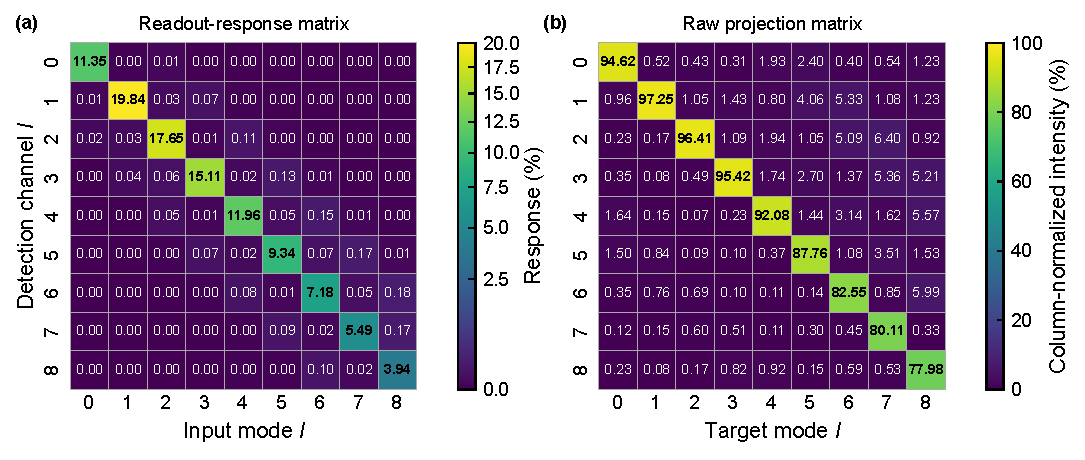
\includegraphics[width=\textwidth]{figures/supplement/figS_readout_response_raw_projection}
\caption{Projection-arm readout response and raw projection data for Run~1. (a) Readout-response matrix $\mathbf{S}$. The diagonal responses span $3.94\%$--$19.84\%$, the maximum off-diagonal response is $0.180\%$, and the condition number is $\kappa(\mathbf{S})=5.05$. (b) Column-normalized raw projection matrix measured for the simultaneous nine-mode input before response correction. Values in panel~(b) are normalized for visualization; the inversion uses the raw detected-power vectors.}
\label{fig:supp_readout_response_raw_projection}
\end{figure}

For the simultaneous nine-mode measurement at locking condition $j$, let $\mathbf{y}^{(j)}$ denote the raw detected-power vector across the nine projection channels and let $\mathbf{x}^{(j)}$ denote the corresponding cavity-output channel weights. Within each experimental run, $\mathbf{S}$ is the run-specific readout-response matrix. The measurement model is
\begin{equation}
\mathbf{y}^{(j)}=\mathbf{S}\,\mathbf{x}^{(j)}.
\label{eq:supp_meas_model}
\end{equation}
The channel-weight vector is estimated by non-negative least-squares inversion~\cite{Rehacek2010}:
\begin{equation}
\hat{\mathbf{x}}^{(j)}=\arg\min_{\mathbf{x}\ge 0}\left\|\mathbf{S}\mathbf{x}-\mathbf{y}^{(j)}\right\|_2.
\label{eq:supp_nnls}
\end{equation}
The estimated vectors are then normalized column-wise so that each column sums to unity. The sorting efficiencies and extinction ratios reported in the main text are calculated from the resulting response-corrected matrix. The three independently measured readout-response matrices have condition numbers from $4.99$ to $5.43$, so the inversion is well conditioned. The calibration and simultaneous nine-mode measurements use the same sequential single-channel projection-arm configuration, so $\mathbf{S}$ is applied under the readout conditions in which it is acquired.

%% ============================================================
\subsection*{B.2 Design-point tolerance at the nine-mode boundary}

Fig.~\ref{fig:supp_tolerance_map} quantifies the robustness of the $M=9$ consecutive design point against deviations $\Delta k$ from the optimum $k^*=2/9$. Panel~(a) plots the minimum resolvability $\tau_{\min}=\mathcal{F}\,s_{\min}$ as a function of $\Delta k$ for the threshold finesse $\mathcal{F}_{\min}=27$ and the measured finesse $\mathcal{F}=32.21$. At $\mathcal{F}_{\min}$, the threshold $\tau_{\min}\ge\tau_0=3$ is satisfied only at the exact optimum. The measured finesse opens a tolerance window $\Delta k\in[-3.6,\,+4.5]\times10^{-3}$ within which $\tau_{\min}$ remains above $\tau_0$. Panel~(b) shows the corresponding system extinction ratio $\mathrm{ER}_{\mathrm{sum}}$ at $\mathcal{F}=32.21$, evaluated from the Airy closed form [Eq.~(\ref{eq:supp_pnoise_closed})]. At the design point $\Delta k=0$, the mean and worst-mode $\mathrm{ER}_{\mathrm{sum}}$ both reach the exact finite-$M$ Airy prediction of $12.04\,\mathrm{dB}$. Both values remain above the conservative lower bound of $10.47\,\mathrm{dB}$ set by the large-$M$ limit throughout the tolerance window.

\begin{figure}[htbp]
\centering
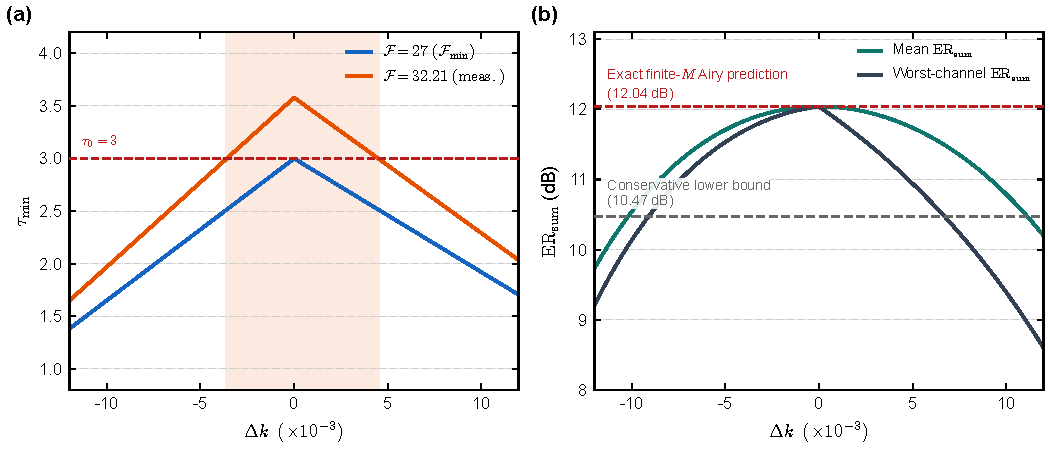
\includegraphics[width=\textwidth]{figures/supplement/figS1_tolerance_map}
\caption{Tolerance of the $M=9$ consecutive design point. (a)~Minimum resolvability $\tau_{\min}$ versus Gouy-step deviation $\Delta k$ at the threshold finesse $\mathcal{F}_{\min}=27$ (blue) and the measured finesse $\mathcal{F}=32.21$ (orange). The shaded region marks the tolerance window where $\tau_{\min}\ge\tau_0=3$. (b)~System extinction ratio $\mathrm{ER}_{\mathrm{sum}}$ versus $\Delta k$ at the measured finesse, showing mean and worst-mode values. The horizontal dashed reference lines mark the conservative lower bound of $10.47\,\mathrm{dB}$ set by the large-$M$ limit and the exact finite-$M$ Airy prediction of $12.04\,\mathrm{dB}$ at the design point $k^*=2/9$.}
\label{fig:supp_tolerance_map}
\end{figure}

%% ============================================================
\section*{Appendix C. Extension to general stable two-mirror cavities}

The main text derives the folding model for a plane-concave cavity. The design analysis, however, depends on the cavity geometry only through the normalized Gouy step~$k$. This section shows that a branch-independent effective step can be defined for a general stable two-mirror cavity. The folding positions, spacing criterion, crosstalk sums, and capacity bound therefore carry over without modification.

Consider a stable Fabry--P\'{e}rot cavity of length $L$ formed by two mirrors with radii of curvature $R_1$ and $R_2$. The standard $g$-parameters are
\begin{equation}
g_1 = 1-\frac{L}{R_1}, \qquad g_2 = 1-\frac{L}{R_2},
\label{eq:supp_g_params}
\end{equation}
The stable regime considered here satisfies $0<g_1 g_2<1$. The transverse-mode resonance frequencies are given by~\cite{Kogelnik1966,Siegman1986}
\begin{equation}
\nu_{q,N} = \mathrm{FSR}\!\left(q + N\frac{\eta}{\pi}\right), \qquad \eta = \arccos\!\bigl(\sigma\sqrt{g_1 g_2}\bigr),
\label{eq:supp_gen_resonance}
\end{equation}
where $\sigma=+1$ for the near-planar branch and $\sigma=-1$ for the near-concentric branch. On the folded circle, steps $k$ and $1{-}k$ give the same set of pairwise arc lengths. The branch-independent effective step can therefore be written as
\begin{equation}
k_{\mathrm{eff}} = \frac{1}{\pi}\arccos\!\bigl(\sqrt{g_1 g_2}\bigr) \in (0,\tfrac{1}{2}).
\label{eq:supp_keff}
\end{equation}
With this replacement, the folded positions $\mathrm{pos}(N)$, pairwise spacings $s_{ij}$, and minimum spacing $s_{\min}$ are determined by the target orders and $k_{\mathrm{eff}}$, rather than by the cavity type itself. The same spacing criterion, crosstalk sums, and capacity bound $M\le\lfloor\mathcal{F}/\tau_0\rfloor$ therefore remain applicable. Only the mapping from $k_{\mathrm{eff}}$ to the geometric parameters changes with cavity type.

\medskip\noindent\textbf{Plane-concave cavity.}\quad
Taking the planar limit $R_1=\infty$ and denoting $R_2=R$ gives $g_1=1$ and $g_2=1-L/R$. Equation~(\ref{eq:supp_keff}) then reduces to $k_{\mathrm{eff}}=\pi^{-1}\arccos\!\bigl(\sqrt{1-L/R}\bigr)$, recovering the main-text formula. The inverse mapping is $L/R=\sin^2(\pi k_{\mathrm{eff}})$.

\medskip\noindent\textbf{Symmetric double-concave cavity.}\quad
For $R_1=R_2=R$, the $g$-parameters satisfy $g_1=g_2=1-L/R$. Equation~(\ref{eq:supp_keff}) becomes
\begin{equation}
k_{\mathrm{eff}} = \frac{1}{\pi}\arccos\!\left(\left|1-\frac{L}{R}\right|\right).
\label{eq:supp_keff_dc}
\end{equation}
Solving for the geometry ratio yields
\begin{equation}
\frac{L}{R} = 1 \pm \cos(\pi k_{\mathrm{eff}}),
\label{eq:supp_dc_inverse}
\end{equation}
where the minus sign corresponds to the near-planar branch ($0<L/R<1$) and the plus sign corresponds to the near-concentric branch ($1<L/R<2$). In this symmetric geometry, the waist lies at the cavity centre and has Rayleigh range $z_R=\frac{1}{2}\sqrt{L(2R-L)}$; by comparison, the plane-concave geometry has $z_R=\sqrt{L(R-L)}$. In the near-planar small-$L/R$ limit,
\begin{equation}
k_{\mathrm{pc}} \approx \frac{\sqrt{L/R}}{\pi}, \qquad k_{\mathrm{dc}} \approx \frac{\sqrt{2L/R}}{\pi} = \sqrt{2}\,k_{\mathrm{pc}}.
\label{eq:supp_small_rho}
\end{equation}
Thus, at the same geometry ratio $L/R$, the near-planar double-concave cavity has a Gouy step larger than that of the plane-concave cavity by a factor approaching~$\sqrt{2}$.

\medskip\noindent\textbf{General asymmetric two-mirror cavity.}\quad
For an asymmetric cavity with $R_1\neq R_2$, the condition $g_1 g_2=\cos^2(\pi k_{\mathrm{eff}})$ yields a quadratic equation for~$L$:
\begin{equation}
L = \frac{R_1+R_2 \pm \sqrt{(R_1+R_2)^2 - 4R_1 R_2 \sin^2(\pi k_{\mathrm{eff}})}}{2}.
\label{eq:supp_general_inverse}
\end{equation}
The smaller and larger roots give the near-planar and near-concentric realizations, respectively. The plane-concave limit and the symmetric double-concave case recover the preceding mappings.

\medskip\noindent\textbf{Branch sensitivity.}\quad
The geometry-to-step derivative provides a local measure of how strongly a given coprime branch responds to fabrication tolerances. For the plane-concave cavity,
\begin{equation}
\left|\frac{dk}{d(L/R)}\right|_{\mathrm{pc}} = \frac{1}{2\pi\sqrt{(L/R)(1-L/R)}}.
\label{eq:supp_sensitivity_pc}
\end{equation}
This sensitivity is minimized at $L/R=1/2$. For the symmetric double-concave cavity,
\begin{equation}
\left|\frac{dk}{d(L/R)}\right|_{\mathrm{dc}} = \frac{1}{\pi\sqrt{(L/R)(2-L/R)}}.
\label{eq:supp_sensitivity_dc}
\end{equation}
The minimum occurs at $L/R=1$, corresponding to the confocal point. As a result, the most robust $M=9$ branch shifts from $m=2$ in the plane-concave geometry to $m=4$ in the symmetric double-concave geometry. The optimal step condition $k^*=m/M$ and the capacity bound $M\le\lfloor\mathcal{F}/\tau_0\rfloor$ remain unchanged; only the geometric realization and the robustness ranking change with cavity type.

\bibliography{bib/refs_local}

\end{document}
